
\begin{figure}
 \centering % avoid the use of \begin{center}...\end{center} and use \centering instead (more compact)
 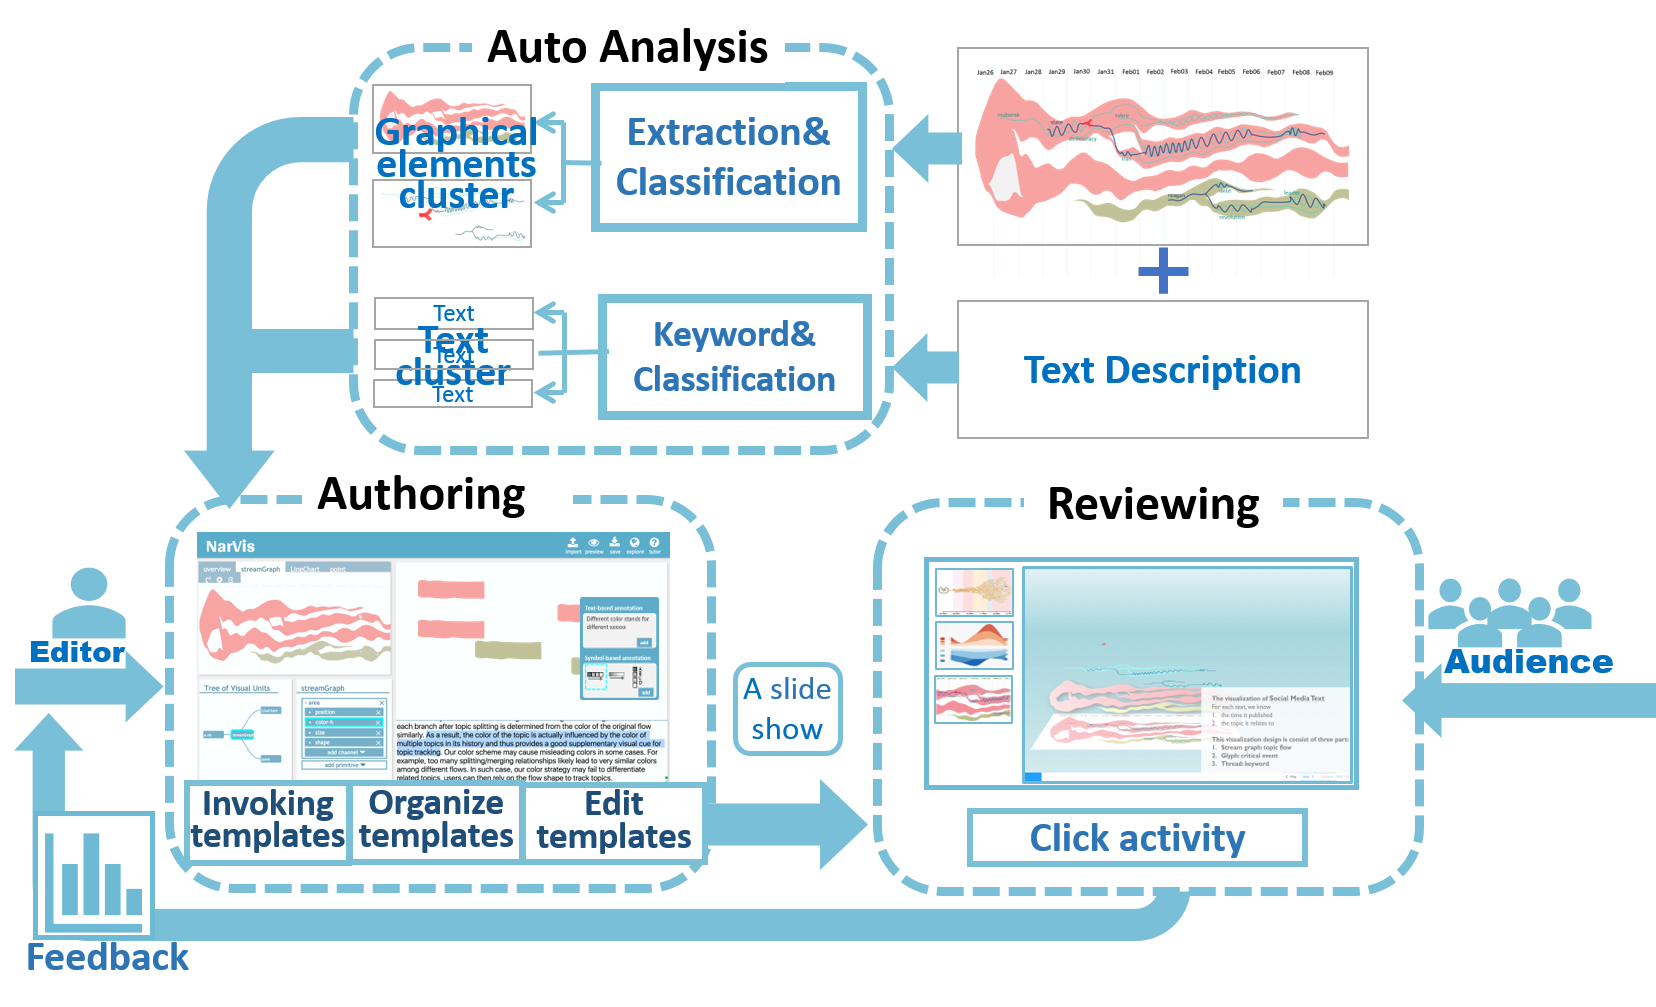
\includegraphics[width=\columnwidth]{overview}
 \caption{An abstract representation of the workflow of Narvis: (i)Auto Analysis; (ii) Authoring; (iii) Reviewing and how the two kinds of users: (i) editors and (ii) audiences, are involved. }
 \label{fig:overview}
\end{figure}


\section{Narvis: System Design and Implementation}

% Thus, it has two kinds of users: editors, the data visualization experts who use Narvis to create an explanation slideshow, and audiences, the general audience who watch the slideshow created by ediors.

Guided by the theory model discussed in Section~\ref{analysis}, as well as the design tasks discussed in Section~\ref{sec:design_task} we design and implement Narvis, an authoring tool for crafting slideshows for the presentation of visualization. The workflow of Narvis consists of three phases (Figure ~\ref{fig:overview}), i.e., Automatic Analysis Phase, Authoring Phase, and Viewing Phase.

% The workflow of Narvis includes three phases (Figure \siwei{ref}):  In Automatic Analysis Phase, the system accepts the input visualization, extracts graphical elements and classifies them into groups for further edit. 
% In Human Editing Phase, editors will be involved to modify the output from the Automatic Analysis Phase, and use the templates Narvis provide to craft a explanation slideshow. 
% In Reviewing Phase, audience can assess the slide show generated in Human Editing Phase. Their click activity and comments will be recorded and send to the editors, helping them improve the quality of the slide show. 



% The auto analysis has two parts: one for input image and one for input text. It automatically extract the graphic elements and divide them into different cluster, facilitating later editing.(DE1) Note that the textual input is not necessary but it provides hints when editors add annotations manually in the Human Editing Phase.(DE1)
\subsection{Phase1: Auto Analysis}
The input of Narvis includes two parts: one image presenting a visual design (mandatory) and a piece of text describing the design (optional). Considering that the vast majority of visualizations are only available as bitmap images, we offer an algorithm to detect and extract the graphical elements from the input image. Here, we explain the basic idea of how Narvis analyzes these input sources to facilitate further authoring. 
%\begin{algorithm} 
%        \caption{Object Detection}  
%        \label{alg:alg1}
%        \begin{algorithmic} % line number
%            \Require A bitmap in the form of a two-dimensional array: $A$
%            \Ensure A list of objects: $B$
%            \State $B \gets \{\}$
%            \ForAll{$pixel (x,y) \in A$} 
%                \If{no mark on $pixel(x,y)$}
%                    \State $Q \gets \{(x,y)\} $
%                    \State $Obj \gets \{\}$
%                    \ForAll{$(x,y) \in Q$}
%                        \State $Q = Q - \{(x,y)\}$
%                        \State $Obj = Obj \cup \{(x,y)\}$
%                        \ForAll {$(x',y')$ which $|x'-x|+|y'-y|\leq2$ and no mark on $pixel(x',y')$}
%                            \If{$pixel(x,y)$ and $pixel(x',y')$ have similar color}
%                                \State $Q = Q \cup \{(x',y')\}$
%                                \State Make a mark on $(x',y')$
%                            \EndIf
%                        \EndFor
%                    \EndFor
%                    \State $B = B \cup \{Obj\}$
%                \EndIf
%            \EndFor
%            \State \Return{$B$}
%        \end{algorithmic}  
%    \end{algorithm} 
%    
    
    \begin{algorithm}  
        \caption{Object Clustering} 
        \label{alg:alg2} 
        \begin{algorithmic} % line number
            \Require A list of objects: $A$, the number of clusters: $N$
            \Ensure A list of objects: $B$
            \State $E \gets \{\}$
            \ForAll{$a_1 \in A$}
                \ForAll{$a_2 \in A$ and $distance(a_1,a_2) \leq L$} \Comment{$L$ is a parameter that accelerates our calculations}
                    \If{$a_1$ and $a_2$ have similar color}
                        \State $d \gets$ the distance between $a_1$ and $a_2$
                        \State $E \gets E \cup \{(a_1, a_2, d)\}$
                    \EndIf
                \EndFor
            \EndFor
            \State $B \gets A$
            \State $E \gets$ sort $E$ by the $d$ of each elements in descending order
            \ForAll{$(a_1,a_2, d) \in E$}
                \State $b_1 \gets b|b\in B, a_1 \subseteq b$
                \State $b_2 \gets b|b\in B, a_2 \subseteq b$
                \If{$b_1 \neq b_2$}
                    \State $B = (B - \{b_1\} - \{b_2\})\cup \{b_1 \cup b_2\}$
                \EndIf
                \If{$|B|\leq N$}
                    \State break
                \EndIf
            \EndFor
            \State \Return{$B$}
        \end{algorithmic}  
    \end{algorithm} 
    
\subsubsection{Analysis of Input Image}
% The auto analysis of input image has three main steps. It first detects all primitives that it finds in the given image and also detects any labels that are present in the visualization. It will then cluster objects that are spacially linked and extract non-target objects. Finally, it will fill in any empty spaces left inside objects from extraction with the appropriate color so as to show the target object in its entirety.
The analysis of the input image includes two steps, object detection and object clustering.
% and object recovery.

% The first step, object detection, is done by iterating through all the pixels on the bitmap. 

\textbf{Object detection.} We iterate through all pixels, and clusters all the pixels that are i) neighbors and ii) have the similar color through a modified breath-first search algorithm. Simple objects, such as a bar in a bar chart, a node in a scatter plot, are detected and extracted after this step.


\textbf{Object clustering.} All the objects with spatial and appearance similarity are clustered to allow an efficient manipulation, as described in Algorithm~\ref{alg:alg2}. For example, all the nodes in a scatter plot should be put in one cluster, instead of letting the editor add them one by one manually.     
%\noindent 
%\textbf{Object recovery.} Once we have completed extraction, we have the issue of these white spaces. The reason this is an issue is because an extracted object might have been dividing two objects, and so when it is extracted, we lose the boundary between our target object and another object, which can cause confusion as to whether that white space should be colored in or not. To solve this boundary problem, we create a queue of the white spaces, with each data point giving the starting and ending point of that space. We then look at the intervals between enclosed white spaced objects, if that interval is above a threshhold, we take that white space to not be part of our object. If it is below our threshhold, then we enclose the white space with the target objects color, creating a boundary for it. The main difference is that for objects not within our target object, we do not create a boundary, whereas objects within our target object are enclosed with the target objects color.

\subsubsection{Analysis of Input Textual Description}
For the inputted textual description, we offer a keyword detection and classification algorithm, which is based on a dictionary of terms that are identified as highly related with visual grammars. e.g. the word ``length'' and ``encodes'', are highly correlated with the  visual grammar of size. We extract all the sentences containing the terms in our dictionary, and cluster them based on the terms they have.

The algorithm we proposed is a compromise between efficiency and performance. It is a heuristic algorithm for images with high quality and clear edges, but its performance can be improved by adopting other well-established algorithms, such as an algorithm based on patch detection and clustering \cite{savva_revision:_2011} and an algorithm based on edge maps \cite{huang2003model}.

\begin{figure}
 \centering 
 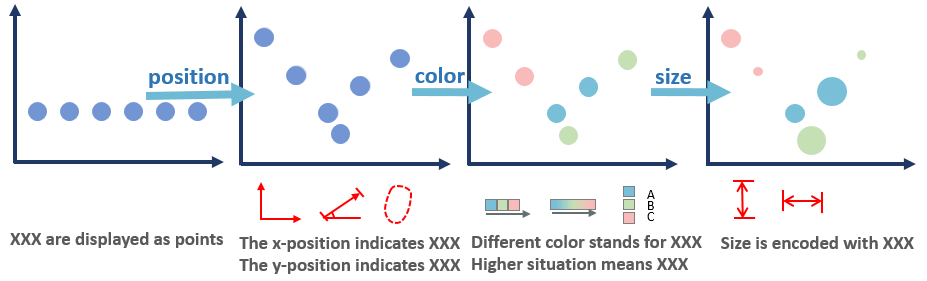
\includegraphics[width=\columnwidth]{tempelate}
 \caption{Demonstration of the template for bubble chart, which is composed of series of slides(top), symbol-based annotation for each visual channel (middle), and text-based annotation for each visual channel(bottom). }
 \label{fig:template}
\end{figure}


\subsection{Phase2: Authoring}
In the Authoring Phase, editors craft an introduction slideshow by constructing built-in blocks called templates in Narvis. We first explain how we design and organize the templates in Narvis, then demonstrate the workflow of this phase, which includes three steps, i.e., invoking templates, organizing templates and modifying templates, as illustrated in Figure~\ref{fig:overview}. 

% We introduce three panels in this phase acting as three steps in the workflow to allow editors  
\subsubsection{A Library of Templates}
We propose a library of templates for the narrative explanation of a visualization. A template is a set of slides that intends to introduce a visual unit. Since an advanced visualization design is the assembly of miscellaneous visual units, such templates can achieve a high level of efficiency for the explanation of a visualization (DA.1). Furthermore, to adapt to various usage scenarios, Narvis allows users to modify and refine templates through rich interactions.


\textbf{Types of templates.}
Narvis organize the provided templates with a 8*3 matrix, where the 3 columns stand for 3 construction rules and the 8 rows stand for  8 visual primitives, as shown in Table ~\ref{tab:unit}. Narvis is extensible, we plan to introduce new templates in the future. At the same time, it is desirable to keep the set of supported marks small and well organized, so as to avoid overwhelming users with a cornucopia of confusing options.


\textbf{Templates design.}
We apply the analysis and theory model in Section~\ref{analysis} for the design of templates. A template has four core components: 1) a well-considered narrative sequence for visual grammar explanation; 2) exaggeration or suppression of certain visual channels in some slides; 3) a series of narrative techniques such as attention cues, animated transitions, information repetition, to orientate visual attention and facilitate perception (DE.1); 4) Hints for adding annotations (DE.2) in each slide. 

With a visual unit, more specifically, a set of graphic elements, as input, a template will generate a slideshow and each slide illustrates one visual grammar(DE.1). These slides are sorted based on the narrative sequence we discussed in section 3.3. In each slide, we offer hints to guide the annotation process (DE.2). These hints are a sentence with blanks to fill in, heuristic questions, or a list of suggestion symbols. A visual channel is suppressed until its grammar has been explained. For example, in Figure~\ref{fig:template}, before we introduce the visual grammar of color, all the object will be blue. The graphical elements in different slides, which have different visual appearances due to the applied exaggeration or suppression of certain visual channels, are perceptively connected through morphing animation. 

\begin{table}[tb]
  \caption{A summary of the animations provided by Narvis}
  \label{tab:animation}
  \small
  \centering
  \begin{tabular}{p{1cm}|p{0.9cm}|p{0.9cm}|p{0.9cm}|p{1.5cm}|p{0.9cm}}
  \toprule
 \textbf{Animation} &\textbf{Engaging} & \textbf{orientate attention} & \textbf{perception} &\textbf{working scenario} &\textbf{ref} \\ 
  \midrule
  \textbf{Morphing} &\checkmark & \checkmark &\checkmark & grammar of size, grammar of shape & \cite{ruchikachorn_learning_2015, heer_animated_2007} \\ 
  \midrule
  \textbf{Blur} &   &\checkmark  &   & focus+context & \cite{pinto2008selecting}\\ 
 \midrule
  \textbf{Flicker} & & \checkmark &  & focus &\cite{waldner_attractive_2014} \\
  \midrule
  \textbf{Motion} & \checkmark & \checkmark & \checkmark & grammar of position & \cite{huber_visualizing_2005} \\
  \midrule
  \textbf{Zoom-in/out} & \checkmark &\checkmark &  & focus&  \\
  \midrule
  \textbf{Annotation} &  & \checkmark &\checkmark &   textual explain & \cite{segel_narrative_2010 } \\
  \midrule
  \textbf{Fade in/out} &  & \checkmark &  & & \\
  \midrule
  \textbf{Decompose} & \checkmark &  &\checkmark & Show how a visualization is composed by visual units & A novel design by us \\
  \bottomrule

  \end{tabular}
  \vspace{1mm}
\end{table}



\textbf{Animation embedded in templates }
Narvis provides 8 types of animation, implement them in templates based on their effects on human attention and perception (DA.1), which has been widely discussed in previous work~\cite{robertson_effectiveness_2008, waldner_attractive_2014, heer_animated_2007}. We also provide a novel decomposition animation, which displays how a visualization is decomposed to several visual units. This animation, at the beginning of the introduction slideshow, aims to engage the audience as well as to help them get a sense of overview (DA.6).
Animation is a double-edge sword, which brings both benefits and pitfalls. We are not discussing its effects here but leave it to the judgment of editors by giving them the freedom to remove it.

     
\begin{figure}
 \centering % avoid the use of \begin{center}...\end{center} and use \centering instead (more compact)
 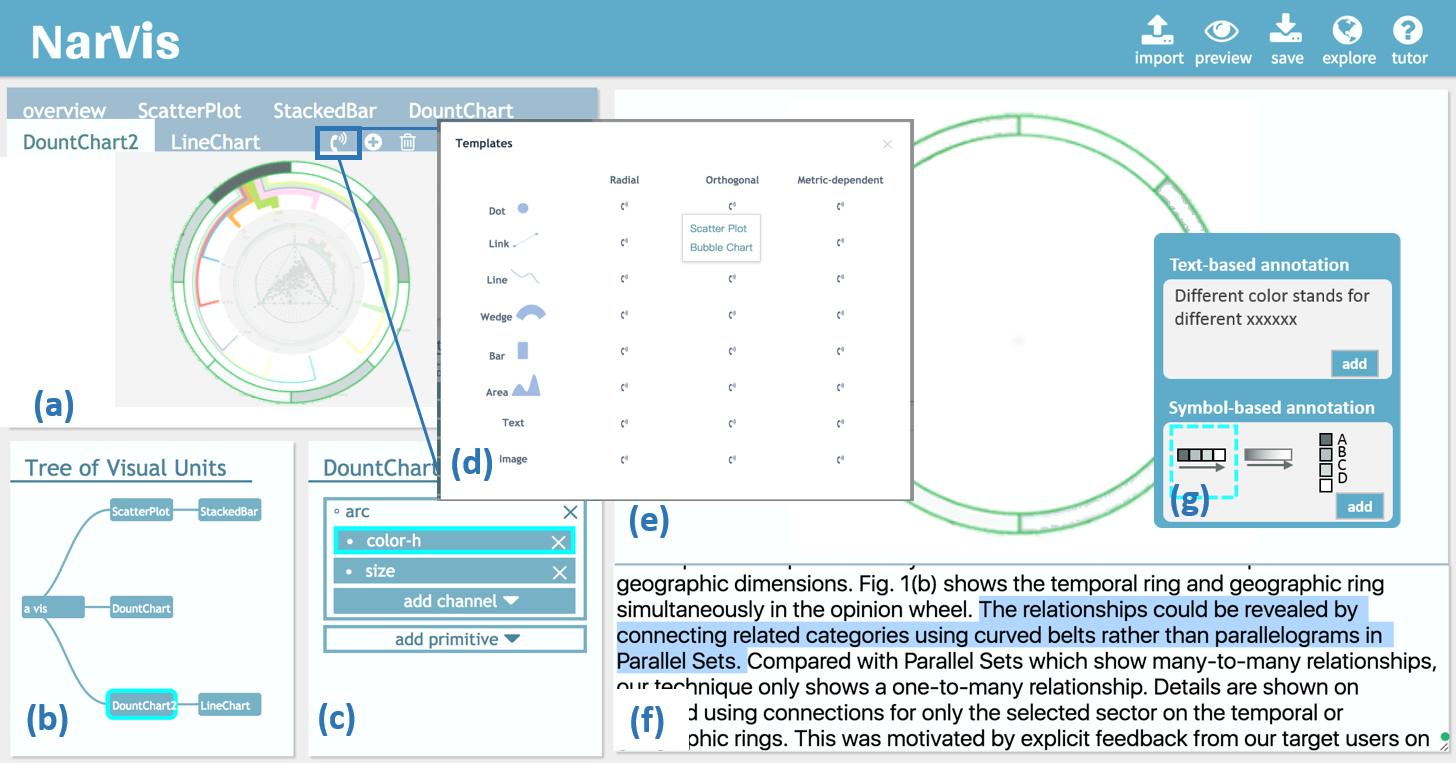
\includegraphics[width=\columnwidth]{interface}
 \caption{Annotated screenshot of the interface of Narvis: a) Source Panel, b) Tree Panel, c) Unit Panel, d) the library of templates, e) Edit Panel, f) text area where the related sentence is highlighted from input textual description, g) a floating annotation window that offers options for adding annotation}
 \label{fig:interface}
\end{figure}   


\subsubsection{Invoking Templates} 

After graphical elements are extracted and clustered based on visual representation, each cluster appears as a tabbed panel in the \textit{Source Panel} (Figure ~\ref{fig:interface}(a)). 

Editors can switch between these tabbed panels, add or delete graphical elements in each panel, making sure that 1) all the graphical elements of the same visual unit are in the same panel; 2) every graphical element belongs to one and only panel. Then, for each visual unit, editors call a template from all the templates provided by Narvis (see in Figure~\ref{fig:interface}(d)). 

The relationship between graphical elements and templates is similar to the one between data and function. Templates contain a set of operations to produce a sequence of slides from the input graphical elements. For example, in Figure~\ref{fig:template}, the ``scatter plot'' templates modify the appearance of the input picture and outputs 4 slides that describe different visual grammars. 

\subsubsection{Organizing Templates} 
Once invoked, a template will show on the \textit{Tree Panel} (Figure ~\ref{fig:interface}(b)) as a tree node. 
By dragging and dropping these nodes, editors organize the structure of the tree diagram, which reflects the relationship between visual units and determines the narrative sequence of the slideshow. This tree diagram will be automatically inserted in the generated slideshow, demonstrating the overall structure to the audience (DA. 6). 

\subsubsection{Modifying Templates} 
% \textbf{\textit{ Unit Panel \& Editor panel}: personalized modification}
% but it also allow the users high flexibity to modify these temples, thus guaranteeing the expressiveness of this system. 
Narvis provides templates to generate slideshows with high efficiency. 
It also supports flexible modification of templates for expressiveness.
Editors can edit a template in the \textit{Unit Panel} (Figure~\ref{fig:interface}(c)) by selecting a node on the \textit{Tree Panel}. In each template, all possible visual grammars are enumerated. Editors can delete unused one themselves, instead of adding the ones used, thus eliminating the unconscious omission of crucial information (DA.5).
It also recommends a narrative sequence of visual grammars, based on the metrics we mentioned in Section~\ref{relationship} (DA.2). 
In the \textit{Editor Panel} (Figure~\ref{fig:interface}(e)), with the hints from Narvis, editors add annotations to facilitate graph and chart comprehension. For each slide, which is defaulted to explain one visual grammar in our templates, Narvis offers questions or sentence with blank for adding text-based annotation and a list of suggested design options for symbol-based annotation (DE. 2) that can be added into the slide by a simple one-click (DE.1), as show in Figure~\ref{fig:interface}(g).



\begin{figure}
 \centering 
 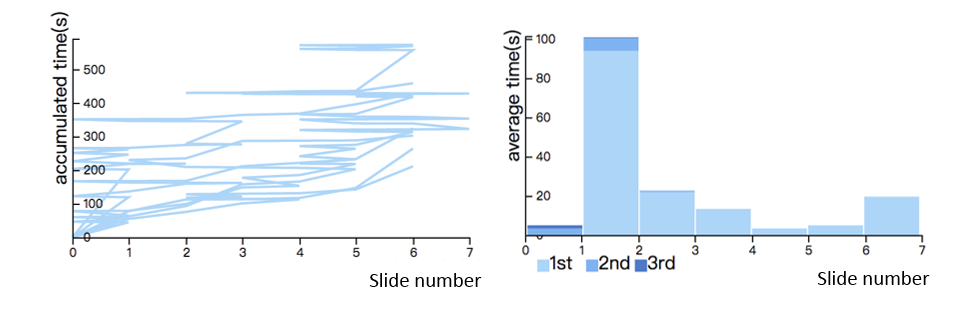
\includegraphics[width=\columnwidth]{feedback}
 \caption{The click stream data of one slideshow visualized as a line chart (left) and a stacked bar chart(right). The x-axis stands for the number of slides. In the line chart (left), the y-axis stands for the accumulated time an audience spent for watching, while in the bar chart (right), the y-axis stands for the average time all audience spent on watching this slide. }
 \label{fig:feedback}
\end{figure}


\subsection{Phase3: Viewing}
The slideshow produced by editors will then be watched by the audiences. By clicking the ``explore'' icon on the right top, audiences will be directed to a new window, where Narvis exhibits all the slideshows produced and uploaded.
Audiences can choose one slideshow for watching, click buttons to move forward or backward to view all the slides it contains. Their click activity will be recorded automatically by Narvis for the analysis of their watching behavior. 

These clickstream data will be visualized in the form of a stacked bar chart and a line chart (see in Figure~\ref{fig:feedback}).  
The \textit{x} axis represents the slide's number in both charts. In the line chart, the \textit{y} axis represents the accumulated watching times, and each line refers to the watching behavior of one individual audience. In the bar chart, the y axis represents the average watching time of all users for a certain slide. Each bar is split into colored bar segments. The bottom bar segment represents the time audience spent the first time for watching this slide, if they go back and watch this slide for the second time, a bar segment with darker color will be placed on the top of the previous one, and so on. 

The line chart emphasizes on the watching behavior of every individual while the bar chart focuses on the description of every single slide. 
%\notsure{do I need this?For example, in Figure~\ref{fig:feedback}, the line chart indicates that some audiences go back frequently while other audiences go through all the slides sequentially. The bar chart indicates that it is the second slide that audience spent relatively longer time to read. Even though the going back behavior is frequent, the time people spent for it is little.} 
With the help of these two charts, the editor is able observe how the audiences watch his slideshow and generates ideas for later revision (DE.3). 

%\subsection{Iterative Design}
%To investigate the usability of Narvis, we invited 4 UGs from diverse backgrounds to watch an introduction slideshow produced with Narvis. 
%Based on their feedback, we iterate over the design of Narvis as follow:
%
%\subsubsection{An Compulsory Introduction}
%In the initial design, an introduction slideshow is purely the combination of templates. In other words, it just explains each visual units after displaying an overview of the visualization. However, the participants complained that they were less motivated to learn a visual design without an awareness of the background. Questions like, \textit{what's the motivation of this visual design}, \textit{what's the dataset}, and \textit{what kinds of problems it can solve} need to be answered before the introduction of this visual design. Thus, we added a compulsory introduction slide at the beginning of each slideshow, which is displayed as a root node of the tree diagram in \textit{Tree Panel}. This slide contains questions that guide the editors to give a brief description of the background.
%\subsubsection{Different Levels of Detail}
%While 3 UGs appreciate this detailed introduction slideshow, and consider the animation applied as engaging and enjoyable. Another UG, who has taken a data visualization course before and is familiar with some visualization designs, thought some slides and animation are redundant. 
%Thus, we offer 3 levels of details which the audience can choose from. The detailed one displays all the animation, the normal ones skip the animation for some simple visual grammar such as color and size, and the abstract one discards all animation and put the annotation for color and size in one slide
 
 
 \begin{figure*}
 \centering % avoid the use of \begin{center}...\end{center} and use \centering instead (more compact)
 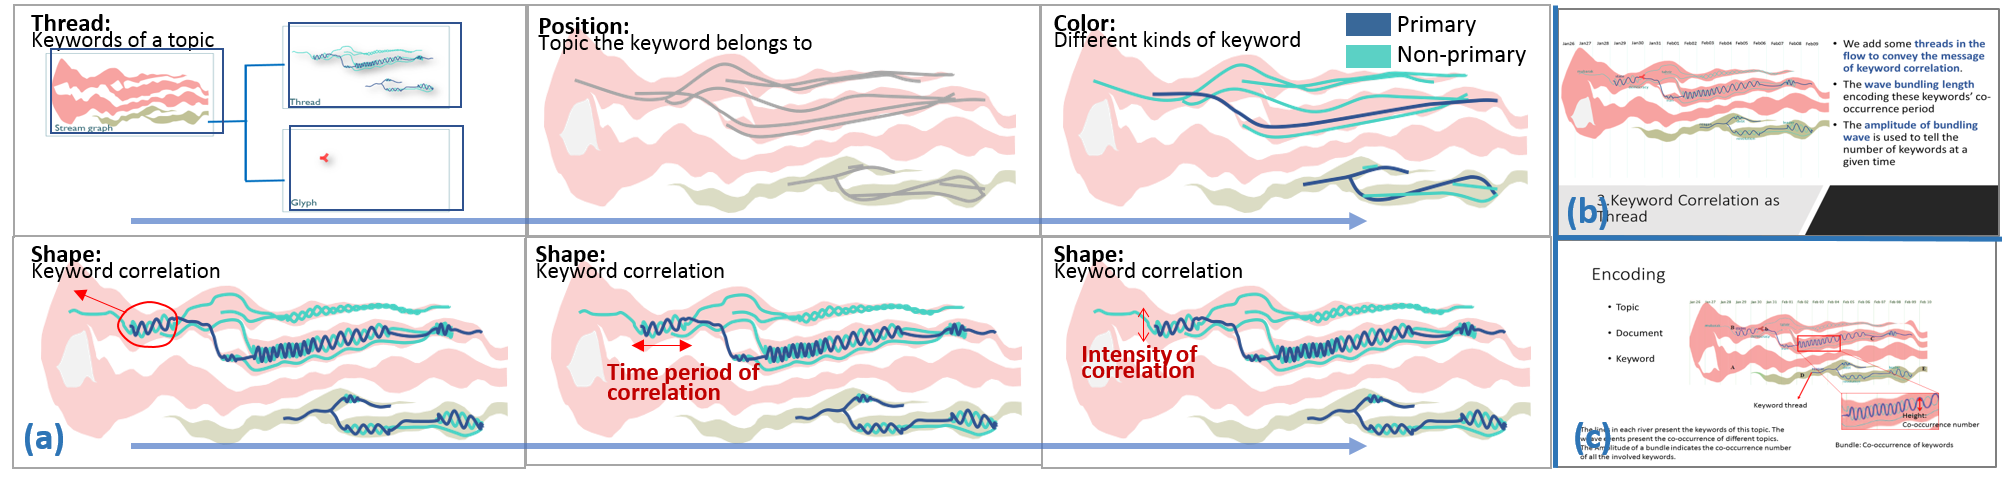
\includegraphics[width=\linewidth]{user_study}
 \caption{The slideshows produced by (a)Narvis and (b),(c)Power Point to introduce a visual unit, thread, in \textit{TextFlow}\cite{cui_textflow:_2011}. Note that (b) and (c) both miss the visual grammar of thread color and (c) forgets to mention the visual grammar of wave bundling length. }
 \label{fig:user_study}
\end{figure*}
 
\subsection{A Working Scenario}
Jessica has extensive experience in the field of data visualization, and has implemented a visual analytics tool for a review service website based on the design of OpinionSeer\cite{wu_opinionseer:_2010}, which has five visual units as demonstrated in Figure~\ref{fig:hierarchic}. To help audiences better understand this design, she needs to publish a tutorial accompanied with it.
First, she loads the screenshot of her system, as well a textual description, into Narvis.
After a few seconds, the system automatically extracts the graphical elements. Jessica first adds five tabbed panels (see in Figure~\ref{fig:interface}(a)), since she identifies five different visual units in OpinionSeer. At each panel, where the uploaded image shows with half-transparency as background, Jessica adds graphical elements by clicking it. As in Figure~\ref{fig:interface}(a)), the ``geometry ring'' is added to a tabbed panel and highlighted. Note that Narvis pre-clusters some graphical elements to convenient the users. For example, all the dots in ``scatter plot'' will be highlighted just by clicking on one dot. 

After some editing, each tabbed panel includes all graphics elements belonging to one visual unit. Now, she chooses templates for each visual unit. 
She first chooses a visual unit by clicking its tab, then clicks the ``phone'' icon. A table (Figure~\ref{fig:interface}(d)) jumps up, which categorizes all the templates as the 8*3 table we described in Section~\ref{compositions}. For example, when Jessica clicks on the (2,1) cell, a dropdown list that contains two templates, the templates for bubble chart and scatter plot, will appear.  

One by one, Jessica invokes 5 templates, all then show as tree nodes in \textit{Tree Panel} as children of the ``a vis'' node. Jessica reorganizes the structure of the tree diagram (see in Figure~\ref{fig:interface}(b)) by dragging and dropping based on her understanding of this visual design. 

Moreover, Jessica edits the narrative templates based on her design. 
% In the templates, we enumerate all the possible visual encodings. 
She goes through all five templates in the \textit{Unit Panel} by clicking the corresponding node in \textit{Tree Panel}, and deletes the visual channels with no encodings, such as the size in the template of scatter plot. 

Jessica further adds annotations at each slide with the help from an annotation window (see in Figure~\ref{fig:interface}(g)). This annotation windows offers some design options for adding text-based annotations as well as symbol based annotations.  The text area Figure~\ref{fig:interface}(f) also offer hints for the addition of annotation by highlight the corresponding textual description. 
% When adding annotation to a certain channel, the related text will highlight in the text area, aiming to offer a better user experience.   


To refine the readability of the tutorial, Jessica asks several friends, who have little experience in data visualization, to watch the tutorial before release. Narvis collects their viewing behavior from click activities, generates statistics results, and visualize it in the form of a stacked bar chart and a line chart (Figure~\ref{fig:feedback}). From these two charts, Jessica finds out that people spent significantly longer time on reading the 4th slide, which points out that information in this slide is not clear or too complicated. Jessica then revises her slideshow accordingly. 



